\section{Information Extraction}
\label{cap2:theoFrame/infExtr}
\subsection{Information Extraction methods with Semantic Web technologies}
\label{cap2:theoFrame/infExtr/methods}
As the Semantic Web aims to make structured data available enabling high levels of 
automation, there are still some challenges regarding the increasing demand for information. 
There is still a gap between the coverage of structured and unstructured data on the 
Web~\cite{infExtr:PolleresHHD10}. However, making high-quality annotations on unstructured 
data is not a trivial task because it requires processing vast amounts of information that 
is constantly changing. 

Thus, automatic techniques for extracting and annotating information have gotten more 
attention in the context of the Semantic Web. As described by Martinez et. al., Information 
Extraction (IE) refers to the automatic extraction of implicit information from unstructured 
or semi-structured sources~\cite{infExtr:MartinezHL19}. IE methods are used to identify 
entities, concepts and/or semantic relations implicit in an input source, typically a text 
in natural language. 

Many systems have been developed to automate the extraction or enrichment of Semantic Web 
resources such as ontologies, knowledge graphs, etc. These systems are often based on 
Information Extraction methods which usually rely on techniques from areas such as Natural 
Language Processing, Machine Learning and Information Retrieval. 

The combination of tools from the Semantic Web and Information Extraction areas presents two 
perspectives: using Information Extraction to populate the Semantic Web, or using Semantic 
Web resources to improve Information Extraction processes. In this work we focus on the last 
perspective mentioned, in particular how to extract and link entities over unstructured input 
sources (such as natural language questions).

An entity is understood as an atomic element within a Semantic Web Knowledge Graph or ontology. 
Entity Extraction \& Linking (EEL) is then the task of identifying mentions in a text or 
document, and linking them as entities to one or more reference knowledge graphs. EEL is 
typically divided into two main steps: a recognition stage where relevant named entities are 
identified, and a disambiguation stage, where entities are mapped to candidate resources in 
the Knowledge Graph and subsequently ranked. Entity extraction often uses off-the-shelf Named 
Entity Recognition (NER) tools to recognise relevant entities. After extraction, Entity 
Linking follows, where the disambiguation of the spotted mentions links each mention to an 
identifier in a target knowledge graph, and may include a score or weight calculation that 
denotes the confidence or support over the output annotations. We now discuss the Entity 
Linking process in more detail.

\subsection{Entity Linking}
\label{cap2:theoFrame/infExtr/entityLinking}
Entity Linking is the task of linking mentions in text to their corresponding entities in a 
Knowledge Graph (e.g. Wikipedia, Wikidata, DBpedia)~\cite{EL:survey-WuHH18}. Aside from 
extracting entities from a knowledge graph, a disambiguation step is also needed. For example, 
for the question \dquotesit{Has Claudio Bravo played for Manchester City FC?}, Entity Linking 
with respect to Wikidata should link the mention \dquotesit{Claudio Bravo} to the Chilean 
football goalkeeper Claudio Bravo (\texttt{wd:Q313161}) instead of the Chilean painter Claudio Bravo 
(\texttt{wd:Q491787}), given the context of the sentence (a person playing in a football club). 
Some applications of Entity Linking involve fields such as information 
retrieval~\cite{infExtr:CornoltiFCRS16, infExtr:BlancoOM15, infExtr:BollegalaMI07} knowledge 
fusion~\cite{infExtr:DongGHHMSZ15, infExtr:BohmFHLMNEHHS12}, or Knowledge Graph 
population~\cite{infExtr:RaoMD13, infExtr:DredzeMRGF10, infExtr:FreedmanMM17}.

Commonly, the entity linking process is divided into three modules: candidate entity 
generation, candidate entity disambiguation and linking the result. A formal description of 
Entity Linking according to Wu and He~\cite{EL:survey-WuHH18} is the following: Given a set of 
documents $d=\{d_1,d_2,\ldots\}$ and a Knowledge Graph $K$, we can get a mention set 
$M=\{m_1, m_2,\ldots\}$ using a Named Entity Recognition tool. For each $m_i \in M$, we can 
get a candidate set $C=\{c_1, c_2,\ldots\}$ from a knowledge base. The goal of Entity Linking 
is to choose an entity from $c \in C$ for each mention $m \in M$. If $score(m,c)$ is below 
$\tau$ ($\tau$ is a threshold) for all $c \in C$, then the target entity of m is 
\textit{Not In Lexicon} (NIL); otherwise, $m$ will be linked to $c'$ such that 
$score(m,c')=max\{score(m,c) \mid c\in C \}$. Figure~\ref{fig:entitylinkingGeneralModel} shows a 
general model including each phase and the formal description mentioned.

\begin{figure}[!h]
    \centering
    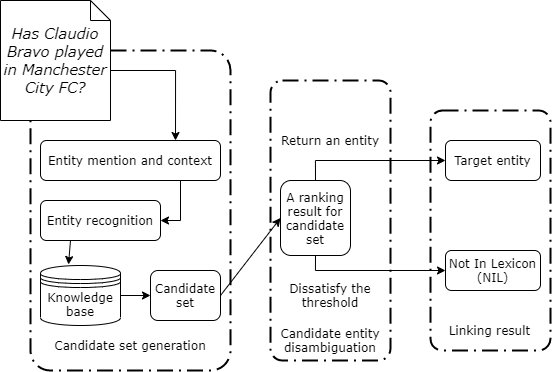
\includegraphics[scale=.5]{imagenes/2_theorical_framework/information_extraction/entityLinkingModel.PNG}
    \caption{A general model of Entity Linking based on Wu and He~\cite{EL:survey-WuHH18}}
    \label{fig:entitylinkingGeneralModel}
\end{figure}

The first module selects the candidate entities for each mention identified in the text and 
finds related entities in the knowledge base. For example, \textit{Claudio Bravo} is related 
to the entities \textit{Claudio Bravo (football goalkeeper)} and \textit{Claudio Bravo (painter)}.

The second module ranks the candidate entities by combining different features of 
entities and assigning scores to each candidate. Some features could be entity popularity, 
entity type, similarity between names or context in the query, topic similarity and a 
combination of several features. In the example, \textit{Claudio Bravo (football goalkeeper)} 
should have a higher score than \textit{Claudio Bravo (painter)} due to the football-related 
context of the sentence. 

The last module selects the target entity for each mention according to the ranking derived 
from the previous module. The candidates with the highest score per mention are selected 
among the candidates whose scores are above the threshold. If scores from all candidates are 
below the threshold, some systems return a NIL clustering~\cite{infExtr:ji2010overview}, 
although we will work with systems that directly discard results that do not satisfy the 
threshold.

There are various existing methods for addressing candidate entity generation and 
disambiguation. The methods for candidate entity generation can be divided into methods 
based on dictionaries~\cite{infExtr:ZhangSTW10, infExtr:HanSZ11}, 
direct search~\cite{infExtr:McNameeMLOD11, infExtr:DredzeMRGF10} and 
probabilistic methods~\cite{infExtr:ganea2016, infExtr:PanCHJK15}. On the other hand, the 
methods for candidate entity disambiguation can be divided into methods based on 
similarity computation~\cite{infExtr:Cucerzan07, infExtr:BunescuP06}, 
machine learning~\cite{infExtr:ganea2016, infExtr:ZhangSTW10} 
and graphs~\cite{infExtr:GongFLSH17, infExtr:HanSZ11}.

One of the main difficulties in Entity Linking is the high ambiguity of entity mentions, 
which make it more difficult to understand the meaning of entity mentions. These ambiguities 
include polysemies, which refer to mentions that correspond to many entities (e.g. 
\textit{Claudio Bravo}) or multiword synonyms, which refer to entities that may have many 
kinds of surface forms (e.g. \textit{Manchester City FC} is also known as \textit{The Citizen} 
or \textit{The Sky Blues}). Another problem happens when selecting entities in the linking 
results phase since the threshold is selected manually and can lead to the problem that 
correct targets can be below the threshold, thus being discarded.

Entity linking evaluation criteria are usually based on Precision, Recall and 
F1-score. For each of these metrics there is a micro measure and a macro 
measure~\cite{entlin:CornoltiFC13}. The macro measure gives equal importance to each 
document since it first calculates the relevant measure over each document, and then 
calculates the arithmetic average. On the other hand, the micro measure considers all 
mentions as part of one document when calculating the relevant measure, thus giving more 
importance to documents with more mentions. The following equations represent the micro and 
macro measures of Precision and Recall:
% E --> G, G --> S
\begin{align*} 
    Precision_{micro} = \frac{|S \cap G|}{|S|} \\
    Recall_{micro} = \frac{|S \cap G|}{|G|} \\
    Precision_{macro} = \frac{\sum_{i=1}^{|D|} \frac{|s_i \cap g_i |}{|s_i|}}{|D|} \\
    Recall_{macro} = \frac{\sum_{i=1}^{|D|} \frac{|s_i \cap g_i |}{|g_i|}}{|D|}
\end{align*}
\noindent where $D$ represents a document containing a number of texts, $G$ is the set of annotated 
entities that should be linked in a document ($g_i$ is the equivalent for each document), 
$S$ the set of linked entities generated by a system in a document ($s_i$ is the equivalent 
for each document). The Precision is the ratio of entities correctly linked to a Knowledge 
Graph over the linked entities generated by a system, while the Recall is the ratio of 
entities correctly linked to a Knowledge Graph over the entities that should be correctly 
linked. Then, the F1-score is a measure that combines Precision and Recall as two 
interacting values and is calculated with the following formula (based on the harmonic 
mean of both measures):

\[
    F1_x = 2 \frac{Precision_x \cdot Recall_x}{Precision_x + Recall_x}
\]
\noindent where $x$ corresponds to the micro or macro version of the F1-score. Aside from Precision, 
Recall and F1-score, some systems also include an Accuracy measure that includes NIL entities, 
though we will not consider this metric in our evaluations as NIL entities in questions 
cannot generate results for queries.

There are many datasets used for evaluation such as KORE50~\cite{entlin:HoffartSNTW12}, 
AIDA-CoNLL~\cite{EL:aida-HoffartYBFPSTTW11}, NEEL~\cite{entlin:RizzoBPV15}, and 
OKE2016~\cite{entlin:Plu0T16}, which can be evaluated over knowledge bases such as Wikipedia, 
DBpedia~\cite{KG:dbpedia}, and YAGO~\cite{KG:yago}. To the best of our knowledge, there is 
no dataset for evaluating Entity Linking over Wikidata, but since Wikidata, DBpedia and 
Wikipedia are all interlinked, we can use datasets with labels for any such resource.

In this work we will use several Entity Linking systems that we will briefly describe later. 
The criteria to choose these systems were: 

\begin{enumerate}
    \item have a public API available that allows at least 10,000 requests per day; 
    \item have references/papers explaining how the system functions; and 
    \item work over either Wikipedia, Wikidata, DBpedia or YAGO. 
\end{enumerate}

Given these criteria, the selected systems are: \textit{DBpedia Spotlight}, \textit{AIDA}, 
\textit{TAGME} and \textit{OpenTapioca}.

\subsubsection{DBpedia Spotlight}
\label{cap2:theoFrame/infExtr/entityLinking/dbpediaSpotlight}
DBpedia Spotlight~\cite{EL:dbpedia-spotlight-MendesJGB11} is a system that automatically 
annotates text documents with DBpedia URIs. The system allows users to configure annotations 
to their specific needs through the DBpedia Ontology and quality measures provided by the 
system. Their approach is divided into four phases.

The \textbf{spotting stage} identifies the phrases in a sentence that may contain a mention 
of a DBpedia resource. Before performing the spotting process, the system builds a lexicon 
of labels extracted using a graph of labels, redirects and disambiguation pages in 
DBpedia. The labels of DBpedia resources are created from Wikipedia page titles, which are 
seen as community-approved surface forms. Redirects to URIs indicate synonyms or alternative 
surface forms (including common misspellings and acronyms) whose labels also become surface 
forms. Disambiguation pages provide links from ambiguous surface forms to the resources they 
potentially link to. The resulting collection of surface forms composes the set of labels for 
the target resources.

As an additional resource for the later disambiguation stage, a collection of occurrences for 
each resource based on wikilinks (page links in Wikipedia associated with one resource) is 
stored as a document in a Lucene\footnote{\url{http://lucene.apache.org}} index.

A \textbf{candidate selection} is then employed to map resource names to candidate 
disambiguations spotted in the previous phase. The DBpedia Lexicalization dataset is used to 
determine candidate disambiguations for each surface form. This phase aims to reduce the 
number of disambiguation possibilities keeping a trade-off between time performance and 
system Recall. 

Following candidate selection is the \textbf{disambiguation stage}, where the system uses 
the context gathered from surface forms to choose the best choice amongst candidates. 
DBpedia resource occurrences are modeled in a Vector Space Model (VSM)~\cite{infExtr:SaltonWY75} 
where each DBpedia resource is a point in a multidimensional space of words. The \textit{Term 
Frequency} (TF) weight and the \textit{Inverse Candidate Frequency} (ICF) weight are 
used to score each candidate. 

The TF weight represents the relevance of a word for a given resource. The ICF weight is 
proposed given that the standard \textit{Inverse Document Frequency} (IDF) 
weight~\cite{infExtr:Jones04} only identifies the global importance for a word, and thus 
fails to capture the importance of a word for a specific set of candidate resources. Instead, 
the ICF weight aims to weight words based on their ability to distinguish between candidates 
for a given surface form. The intuition behind the ICF formula is that the discriminative power 
of a word is inversely proportional to the number of DBpedia resources it is associated with. 

Having the VSM representation of DBpedia resources with $TF \ast ICF$ weights, the 
disambiguation process is performed by ranking candidate resources using the cosine 
similarity score between their context vectors and the context surrounding the surface form.

Finally, annotations can be customized through \textbf{configuration parameters} in order to 
tune parameters to a specific task. The offered configuration parameters can be used to 
allow/deny URIs with some classes or its subclasses, set a required minimum of inlinks, 
establish thresholds to prioritise resources relevant to the topic, reduce highly ambiguous 
resources, and configure a disambiguation confidence to keep a good trade-off between avoiding 
incorrect annotations and losing correct annotations.

A web-service\footnote{\url{https://www.dbpedia-spotlight.org/}} is available for integration with 
external web processes. The service is implemented through RESTful and SOAP web services for 
the annotation and disambiguation processes, and supports various output formats (HTML, XML, 
JSON or XHTML+RDFa).

\subsubsection{AIDA}
\label{cap2:theoFrame/infExtr/entityLinking/aida}
The Accurate Online Disambiguation of Named Entities (AIDA)~\cite{EL:aida-HoffartYBFPSTTW11,EL:aida-tool-YosefHBSW11} 
is an online tool that performs entity detection and disambiguation over the YAGO Knowledge 
Graph. The system's approach combines the use of a Named Entity Recognition (NER) tool with a 
graph-based mapping. 

The system automatically detects mentions using the Stanford NER 
Tagger\footnote{\url{https://nlp.stanford.edu/software/CRF-NER.shtml}} based on a Conditional Random 
Fields (CRF) Classifier~\cite{entLin:FinkelGM05}. Their approach uses Gibbs sampling to identify 
non-local structures while preserving tractable inference by simulated annealing in place of 
Viuterbi decoding in sequence models. They use this technique to improve an existing CRF-based 
information extraction system with long-distance dependency models.

The collection mapping relies on a graph constructed with mentions and their candidate entities 
as nodes and two types of edges: \textit{mention-entity edges} and \textit{entity-entity edges}. 
The \textbf{mention-entity edges} are weighted edges between mentions and their candidates 
entities (one edge per candidate) and represent the similarity between the context of each node. 
The \textbf{entity-entity edges} are weighted edges between different entities and represent the 
coherence, i.e. the semantic relatedness between both nodes.

The \textit{similarity} between a mention and a candidate entity is defined as the linear 
combination of the \textit{prominence} of an entity and the \textit{context similarity} between 
a mention and a candidate entity. The \textbf{prominence} (or popularity) of an entity is 
calculated using the frequency of Wikipedia-based link href anchor texts and links referencing 
the entity. The \textbf{context similarity} is calculated in different ways for a mention's 
context and an entity's context. 

The context of a mention simply considers all tokens in the document as the 
context~\cite{infExtr:ThaterFP10}. For the context of an entity, the system considers entity 
keyphrases, which are pre-computed phrases derived from link anchors in Wikipedia articles that 
entities connect to~\cite{infExtr:ThaterFP10}. These include phrases in the entity article that 
contain category names, citation titles, external references or titles of incoming links. This 
process forms a keyphrase set $KP(e)$ for each entity $e$. 

The \textit{Mutual Information} (MI) measure, which quantifies the \dquotes{amount of information} 
one random variable obtained from observing another one, is used to quantify the specificity weight 
of a keyword with regard to an entity. In this context, the MI for each keyword $w$ is based on 
a joint probability $P(e, w)$ that reflects the probability of $w$ to be contained in either the 
keyphrase $KP(e)$, or any of the keyphrase sets of entities linked to $e$. 

Since keyphrases can rarely match multi-word keyphrases (e.g. the phrase \dquotesit{Nobel Prize 
winner} may occur in the form of \dquotesit{Nobel winner}), a partial-match model is added to 
improve coverage~\cite{infExtr:taneva2011}. This model match individual words and rewards their
proximity. Following this approach, a phrase's cover is computed for each keyphrase, which 
consists of the shortest window of words that maximize the number of words of the keyphrase. 
For example, the text \dquotesit{winner of many prizes including a Nobel} the cover length of the 
keyphrase \dquotesit{Nobel award winner} is 7. Then, the partial-match score of a phrase in a text 
is calculated using the MI weights of the keyphrase words in the phrase and the ones
included on the phrase's cover.

Lastly, the similarity score between a mention and a candidate entity is computed by summing all 
the partial matching scores of the phrases that are part of the keyphrase $KP(e)$.

The \textbf{coherence} weight between a pair of entities is calculated using the number of 
incoming Wikipedia links that both entities share in their Wikipedia articles, which are denoted 
using crossreferencing properties such as \textit{same-as}. This approach is polished up by 
considering the total number of entities in the Wikipedia collection~\cite{infExtr:MilneW08}.

Having built the weighted graph, the system aims to provide an output graph which consists of 
the graph reduced to a dense subgraph where each mention is connected to only one candidate 
entity. The concept of density refers to the minimum weighted degree in the subgraph. The 
calculation of this subgraph is computed using a greedy algorithm where its main loop performs 
two main steps in each iteration: (1) identify the entity node with the lowest weighted degree 
and (2) remove this node and its incident edges only if it is not the last remaining candidate 
entity for one of the mentions. 

AIDA provides a HTTP JSON web service\footnote{\url{https://www.mpi-inf.mpg.de/departments/databases-and-information-systems/research/ambiverse-nlu/aida}} for annotating texts. It can be accessed via CURL requests and only needs to be provided by the 
text that needs to be annotated.

\subsubsection{TAGME}
\label{cap2:theoFrame/infExtr/entityLinking/tagme}
The TAGME system permits augmenting plain-text with hyperlinks to Wikipedia 
pages~\cite{EL:tagme-FerraginaS10}. It can work over short and poorly composed texts. The system 
annotation is divided into three phases.

The first stage includes generating an anchor dictionary based on Wikidata pages. An anchor 
(also referred to as a spot) for a page $p$ is defined as the text used in the hyperlink of 
another page to refer to $p$. These anchors are extracted from Wikipedia pages and also include 
titles of redirect pages and other variants~\cite{entLib:Cucerzan07}. The anchors composed by 
one character or just numbers and anchors with low-frequency are removed. The set of all 
Wikipedia pages linked by a given anchor $a$ is denoted as $Pg(a)$. The final anchor dictionary 
is indexed using Lucene. 

Then, each annotation of an anchor $a$ with some page $p_a \in Pg(a)$, denoted 
$a \rightarrow p_a$, forms what the authors refer to as a \textit{sense}\footnote{For example, 
a mention of Gabriela Mistral on any given Wikipedia article, \dquotesit{Gabriela Mistral} is the 
anchor, and two possible senses are \url{https://en.wikipedia.org/wiki/Gabriela\_Mistral} or 
\url{https://en.wikipedia.org/wiki/Museo\_Gabriela\_Mistral.}}. These senses are built using all 
Wikipedia pages but discarding disambiguation pages, list pages and redirect pages, also indexed 
by Lucene. These results are indexed in a link-graph using 
Webgraph\footnote{\url{http://webgraph.dsi.unimi.it}}.

Often an anchor $a$ has more than one candidate sense, so a disambiguation process is performed. 
Having the set of all anchors contained in a text $T$ denoted by $A_T$, the system tries to 
disambiguate each anchor $a \in A_T$ by computing a score for each possible sense 
$p_a \in Pg(a)$. This process is implemented using a voting scheme that computes for each other 
anchor $b \in A_T \backslash \{a\}$ its vote for the annotation $a \rightarrow p_a$.

To disambiguate the anchor $a$, a ranking process is designed to select its best annotation 
$a \rightarrow p_a$. The TAGME system presents two variants for the ranking algorithm: one based 
on a classifier (DC) and the other based on a threshold (DT). DC uses as features the score 
$rel_a(p_a)$ and the commonness $Pr(p_a|a)$ to train a classifier to calculate the 
\dquotesit{probability of correct disambiguation} for all senses $p_a \in Pg(a)$. The $p_a$ 
reporting the highest classification score is selected. The other approach, DT, computes the 
top-$\epsilon$ best senses $p_a' \in Pg(a)$ according to their $rel_a(p_a')$ score and then 
annotates $a$ with the sense that obtains the highest commonness amongst them. For time 
performance optimization, both variants discard senses with a commonness below a certain 
threshold $\tau$.

Finally, in the anchor pruning stage, the set $M(A_T)$ of candidates produced in the previous 
stage are pruned to avoid meaningless anchors. A \textit{bad anchor} is defined by a score 
computed using two features: the link probability $lp(a)$ of the anchor $a$ and the coherence of 
its candidate senses with respect to the candidate senses of other anchors in 
$M(A_T)$~\cite{infExtr:MilneW08}. This link probability $lp(a)$ corresponds to the ratio between 
the number of times the phrase $a$ occurs as an anchor in Wikipedia, and the frequency with which 
this phrase occurs in both anchor and non-anchor occurrences.

The \textit{coherence} between two candidate annotations is equivalent to the process followed 
in the AIDA system. A score $\rho(a \rightarrow p)$ is then calculated per candidate annotation, 
which is compared to a threshold $\rho_{NA}$, so annotations with a score lower than the given 
threshold are pruned by setting $a \rightarrow NA$ (a fake page to denote pruned annotations). 
Two approaches that combine $lp$ and coherence are presented to compute this score: one is an 
average between the two features and the second is a linear combination trained via linear 
regression.

A web-service hosted by D3Science Infrastructure\footnote{\url{https://sobigdata.d4science.org/web/tagme/tagme-help}} 
is available to annotate text. The system allows to set a threshold $p$ used for discarding 
annotations.

\subsubsection{OpenTapioca}
\label{cap2:theoFrame/infExtr/entityLinking/openTapioca}
OpenTapioca is a lightweight Named Entity Linking system that works over 
Wikidata~\cite{EL:opentapioca-Delpeuch19}, and is restricted to people, locations and 
organizations. Let D be a document; a spot $s$ is a pair of start and end positions in $D$. 
This spot defines a phrase $d_s$ in $D$, and a set of candidate Wikidata entities $E_s$. The 
OpenTapioca system is based on a binary classifier that predicts for each spot $s$, and each 
candidate entity $e$ linked to that spot, if $s$ should be linked to $e$. This approach 
combines \textit{local compatibility} and \textit{semantic similarity} to classify entities 
according to their context.

The \textbf{local compatibility} for an entity $e$ with a phrase $d_s$ is represented by a 
vector of features that considers the popularity of the entity and the commonness of the 
phrase. The popularity of an entity is estimated by a log-linear combination of its number of 
statements $n_e$, site links $s_e$ and its PageRank $r(e)$ (calculated using Wikidata 
statement values and qualifiers as edges). The commonness of a phrase is estimated using a 
unigram language model trained from Wikidata item labels.

Since the aforementioned features do not consider the context of the mention, a graph is defined 
whose nodes are the candidates entities and edges link semantically related entities. The 
approach consists of finding a combination of candidate entities which are both highly 
compatible and densely related in the graph.

Along these lines, the \textbf{semantic similarity} measure is used to make the process 
context-sensitive. An adaptation of the Han et al.'s~\cite{infExtr:HanSZ11} approach is 
proposed, where a similarity metric $sim(e,e')$ is defined for each pair of entities $(e,e')$ 
that defines the probability that two random walks starting from $e$ and $e'$ end up on the 
same item.

Next, a weighted graph $G_D$ is built where each vertex is a pair $(s,e)$ such as $d_s \in D$ 
and $e \in E_s$. A maximum distance $\rho_{max}$ is fixed for edges so a pair of vertices can 
only be linked if its distance is less than or equal to $\rho_{max}$, and both vertices are 
referring to a different mention. The weight is defined for each edge, which is proportional to
the smoothed similarity between entities, discounted by the distance between mentions. The 
weighted graph $G_D$ is represented by a column-stochastic matrix $M_D$ which is an adjacency 
matrix normalized by its columns to sum to one.

The resulting matrix $M_D$ defines a Markov chain on the candidate entities that is used to
propagate the local evidence, which helps to classify entities according to the context. A 
Markov chain is a mathematical model used to model transitions from one state to another, 
usually in a stochastic way. One particularity of Markov chains is that the stochastic 
process is \dquotes{memoryless}. That is, the probability of transitioning to any particular state 
depends solely on the current state and time elapsed\footnote{One example of a Markov chain 
process is the probability question of getting a certain color ball from a bag of balls, when 
replacement is allowed each time a ball is drawn.}.

Then, instead of combining the local features into a local evidence score as done by 
Han et al.~\cite{infExtr:HanSZ11}, each local compatibility feature is propagated 
independently along the Markov chain. This allows for recording the features at each step, 
which defines a vector of features more sensitive to the context while keeping the number of 
features small. Finally, a linear support vector classifier is trained on these features, 
which defines the final score of each candidate entity. For each spot, the system picks the 
highest scoring candidate that the classifier predicts, if any.

OpenTapioca is available through a web-service\footnote{\url{https://opentapioca.org/}} 
implemented using Solr\footnote{\url{https://lucene.apache.org/solr/}} and some Python libraries. 
Its service keeps synchronous with Wikidata in real time.

\subsection{Sequence Labeling}
\label{cap2:theoFrame/infExtr/sequenceLabeling}
Another application of Information Extraction methods is Sequence Labeling~\cite{seqlab:Graves2012-385, seqlab:MaH16}, 
also known as Semantic Role Labeling~\cite{seqlab:GildeaJ02}. Sequence Labeling is a 
semantic analysis tool that can be used to detect meaningful entities, relationships or 
semantic properties in a given sentence. For example, for the sentence \dquotesit{Barbara lives 
in Santiago}, the name \textit{Barbara} could be identified as the subject of the sentence 
or as a person, while the name \textit{Santiago} could be recognized as the object of the 
sentence or as a location.

Some traditional sequence labeling models are based on linear statistical models such as 
Hidden Markov Models~\cite{seqlab:RatinovR09} or Conditional Random 
Fields (CRF)~\cite{seqlab:PassosKM14, seqlab:LuoHLN15}, which mainly rely on hand-crafted 
features and thus are difficult to adapt to new tasks or new domains~\cite{seqlab:MaX14}. 
On the other hand, recent works that combine Neural Networks and Word Embeddings have been 
broadly used to enhance sequential data modeling~\cite{seqlab:ChoMBB14, seqlab:GersSC00}. 
The combination of these two components have shown better results on many Natural 
Languages Processing (NLP) tasks such as POS tagging~\cite{seqlab:MaH16,seqlab:HuangXY15}, 
Named Entity Recognition~\cite{seqlab:ChiuN15,seqlab:HuMLHX16} or Speech 
Recognition~\cite{seqlab:GravesMH13}, mainly due to its capacity to learn and generalize 
with information learned from unlabeled data, which reduces the ambiguity issues that 
previous statistical models suffer from~\cite{seqlab:MaX14}.

In particular, we are interested in Sequence Tagger systems which, given a sequence of 
words, provide a semantic meaning to words or composed words in the context of a given 
corpus. This semantic meaning varies depending on the task. For example, in Part-of-Speech 
(POS) tagging, words in a sentence are usually tagged as nouns, verbs, adjectives, adverbs, 
etc. Another area of use is Name Entity Recognition (NER), where the sequence tagger can 
identify entity names and tag them as person, location, organization, etc. 

Then, the information output by the tagger can be used in other IE methods such as Entity 
Linking. The task fulfilled by the tagger can be adapted depending on the labels used 
(e.g. provide more entity types for NER) but the process of training and learning such 
labels should not change. We will apply these methods later to identify which sequences of 
terms in the question text refer to which elements of the query. The labels output by the 
system are usually known as BIO labels (where BIO means beginning-inside-outside) and 
demark a tag for a word and whether a word is the beginning of a tag, an inside part of a 
tag, or a word outside a tag. An example of a BIO label output can be seen in 
Figure~\ref{fig:flairArchitecture}.

The performance of a Sequence Tagger is measured using a per-word accuracy~\cite{seqlab:MarcusSM94}. 
Let $W=(w_0,\ldots,w_n)$ denote a sequence of words, $(l_0,\ldots,l_n)$ a sequence of 
expected BIO labels and ($(l_{0}',\ldots,l_{n}')$ a sequence of BIO labels output by a Sequence 
Tagger; a word $w_i$ would be labeled correctly if its expected label $l_i$ matches with the label 
$l_{i}'$ delivered by the Sequence Tagger. Then, the Accuracy over $W$ will be $accuracy(W)=
\frac{\mbox{\#words correctly labeled}}{\mbox{total \# words}}$.

In this work, we will use the Flair Framework~\cite{seqlab:flair-AkbikBBRSV19}, which provides 
up-to-date state-of-the-art language models and word embeddings in a simple interface. Flair is 
implemented on Python using the Pytorch framework for implementing Neural Network based models. 
One of the tools Flair provides is a Sequence Tagger model, which includes pre-trained models or 
the capacity of training a new model by providing training data. In order to understand how the 
Flair Sequence Tagger works, we will explain its two main components: Contextual String 
Embeddings~\cite{seqlab:contextual-emb-AkbikBV18} and its main architecture based on a 
Bidirectional LSTM-CRF model.

\subsubsection{Contextual String Embeddings}
\label{cap2:theoFrame/infExtr/sequenceLabeling/contextualEmbeddings}
The construction of Contextual String Embeddings (aka Flair embeddings) is based on two 
Language Models (LM) where each one captures semantic-syntactic information for each word in 
the sentence; one model captures information from the \dquotes{past} and the other model from 
the \dquotes{future} of each word. The information from both models is combined to construct 
representations of words based on their surrounding context.

\paragraph{Language Models} 
\label{cap2:theoFrame/infExtr/sequenceLabeling/contextualEmbeddings/languageModel}
\mbox{}\\
\mbox{}\\
A Language Model (LM) is a probability distribution over sequences of words~\cite{seqlab:PonteC98}. Language models can be character-level or word-level, where the difference lies in the atomic 
unit selected for the language model~\cite{seqlab:PonteC98}. In this work we focus on character-level LMs.

For a character-level LM, 
the goal is to predict the expected character given a set of characters as context, i.e., to 
provide a good distribution $P(x_{0:T})$ over sequences of characters 
$(x_0, x_1,\ldots,x_T)$~\cite{seqlab:Graves13}. Intuitively speaking, we aim to respond to the question: 
\textit{given a certain sequence of characters, what is the most probable character that follows to that sequence?} (e.g. if we provide with the sequence \dquotes{goalkeepe}, it is very likely that the character \squotes{r} should come next). Then, if the objective is to predict the next character given the previous characters, we will train a language a model to learn $P(x_t|x_0,..., x_{t-1})$, for $0 < t <= T$, which gives an estimate of the predictive distribution over the next character given the previous characters. 

Recent work on language models prefers architectures based on Recurrent Neural Networks~\cite{seqlab:contextual-emb-AkbikBV18}. 
Language models based on Neural Networks, also known as Neural Language Models, have shown 
better results than statistical language models~\cite{seqlab:Graves13}, mainly because 
statistical models decrease their performance when dealing with large vocabulary size, which 
causes a data sparsity problem~\cite{seqlab:Egghe07a} (therefore their capacity to generalize 
is limited). 

Among many applications of neural language models, a key application is the creation of word embeddings, which are vector representations of words typically based on the trainable weights within the Neural Networks used in the language model. Word embeddings are 
particularly useful to encapsulate the semantic attributes of abstract concepts (e.g. we can capture to certain extend that \squotes{red} is a color, thus providing a degree of semantic similarity with other colors' embeddings), and such knowledge can be transfer to other tasks in order to enhance other models' learning capabilities (as we will do here for the Sequence Labeling task). In this case, the architecture used to construct Flair embeddings is the LSTM variant~\cite{seqlab:HochreiterS97,seqlab:Graves13,seqlab:ZarembaSV14} which enhances the ability to encode long-term dependencies with its hidden states (weights in an LSTM 
architecture).

\paragraph{Extracting Flair Embeddings}
\label{cap2:theoFrame/infExtr/sequenceLabeling/contextualEmbeddings/flairEmbeddings}
\mbox{}\\
\mbox{}\\
As mentioned earlier, the goal of a character-level language model is to estimate the 
distribution $P(x_{0:T})$ over a sequence of characters $x_0:T =(x_0, x_1,\ldots, x_T)$. This 
results in a joint distribution over the entire sentence, which is the product of the 
conditional probability $P(x_t|x_0,..., x_{t-1})$ of each character of the sentence:

\begin{equation} \label{eq:flairProb}
    P(x_0) = \prod_{t=0}^{T} P(x_T|x_{0:t-1})
\end{equation}

In an LSTM architecture, the conditional probability $P(x_i|x_0,\ldots,x_{i-1})$ is approximated 
as a function of the network output $h_t$:

\[
    P(x_T|x_{0:t-1}) \approx \prod_{t=0}^{T} P(x_T|h_t;\theta)    
\]

\noindent where $h_t$ represents the past context of the character sequence and is computed recursively 
using an additional memory cell $c_t$:

\begin{align*}
    h_t(x_{0:t-1})=f_h(x_{t-1},h_{t-1},c_{t-1};\theta) \\
    c_t(x_{0:t-1})=f_c(x_{t-1},h_{t-1},c_{t-1};\theta)    
\end{align*}

\noindent where $\theta$ denotes all the parameters of the model. The proposed model includes a fully 
connected softmax layer on top of $h_t$, so the likelihood of every character is given by:

\[
    P(x_t|h_t;V) = \frac{exp(V h_t+b)}{\| exp(V h_t+b) \Vert }
\]

\noindent where $h_t^b$ is denoted as the hidden states of the backward model calculated the same way as 
Equation~\ref{eq:flairProb}. We also denote $h_t^f$ as the hidden states $h_t$ of the forward model. 

Finally, output hidden states from both models are concatenated to form the final embedding 
which represents the surrounding context of a word itself. Formally, the contextual string 
embedding of a word-string that begins at character inputs with indices $t_0,t_1,\ldots,t_n$ 
is defined as:

\[
    w_i^{CharLM} := \begin{bmatrix} h_{t_{i+1}-1}^f \\ h_{t_{i}-1}^b \end{bmatrix}
\]

The result are Contextual String Embeddings capable of producing different representations for 
the same lexical word string in different contexts while capturing the semantics of contextual 
use together with the word itself. These embeddings are then used to boost standard Sequence 
Labeling models as explained next.

\subsubsection{Sequence Labeling Architecture}
\label{cap2:theoFrame/infExtr/sequenceLabeling/architecture}
Though the Flair framework supports various sequence tagging models, the default is to use the 
model based on a Bidirectional LSTM with a Conditional Random Field layer on top of the final 
BiLSTM layer, also known as BiLSTM-CRF~\cite{seqlab:HuangXY15}. Let us denote by $w_o,w_1,\ldots,w_n$ 
the input of the model; then we have that:

\[
    r_i := \begin{bmatrix} r_i^f \\ r_i^b \end{bmatrix}
\]

where $r_i^f$ and $r_i^b$ are the forward and backward output states of the model. The final 
sequence probability is then given by a CRF over the possible labels $y$:

\[
    \widehat{P}(y_{0:n}|r_{0:n})\propto \prod_{i=1}^n exp(W_{(y_{i-1},y_i)} r_i +b_{(y_{i-1},y_i)})
\]

The component that improves the performance of these BiLSTM-CRF models is the addition of 
stacked embeddings, which are a combination of different types of embeddings. The way to combine 
each embedding vector is by concatenating them to form a final word vector representation. The 
final word representation chosen in this work is given by:

\begin{equation} \label{eq:flairWordRepr}
    w_i := \begin{bmatrix} w_i^{CharLM} \\ w_i^{GloVe} \end{bmatrix}
\end{equation}

\noindent where $w_i^{GloVe}$ is a precomputed GloVe embedding~\cite{seqlab:PenningtonSM14}. 

\begin{figure}[!h]
    \centering
    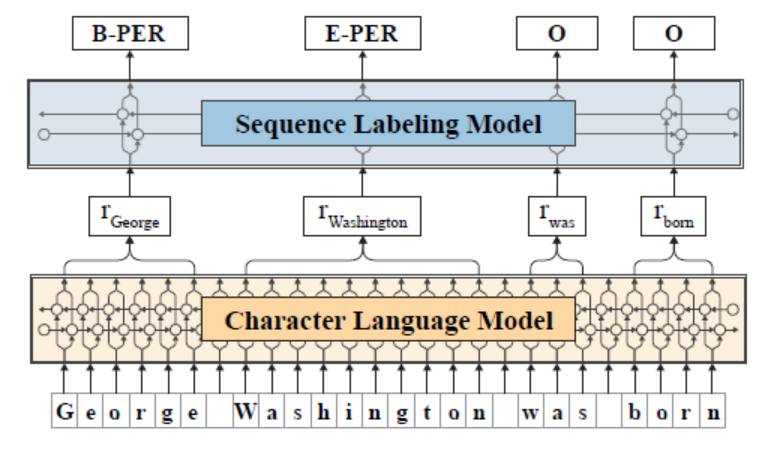
\includegraphics[scale=.5]{imagenes/2_theorical_framework/information_extraction/sequenceLabelingModel.PNG}
    \caption{Flair Sequence Labeling architecture~\cite{seqlab:flair-AkbikBBRSV19}.}
    \label{fig:flairArchitecture}
\end{figure}

Note that these word representations are the input words for the BiLSTM-CRF. An example is shown in 
Figure~\ref{fig:flairArchitecture}, where the Character Language Model mentioned before is fed 
the sentence \dquotesit{George Washington was born} as a sequence of characters. The output 
delivered by the Language Model corresponds to the vector representation of each word following 
Equation~\ref{eq:flairWordRepr}. Then, these sequences of words are taken by the Sequence 
Labeling Model, which gives an output of a sequence of BIO labels such as to indicate that 
the phrase \dquotesit{George Washington} is tagged as a person (PER).
